\begin{frame}
    \frametitle{Dr. Helga}
    \begin{columns}[T]
        \begin{column}{0.55\textwidth}
            \begin{itemize}
                \item Internet Cat-lady since 2012
                \item IRL Cat-lady since 2017
                \item PhD in Computational Engineering
                \item Podcast host and producer of ÍSKISUR (2016-2020)
                \item Previously Research Scientist at deCODE Genetics, Data Scientist at CCP Games
                and Head of AI Research at Travelshift
                \item Currently working as a Postdoc at the University of Iceland
                \item @tungufoss on Twitter
            \end{itemize}
        \end{column}
        \begin{column}{0.4\textwidth}
            \centering
            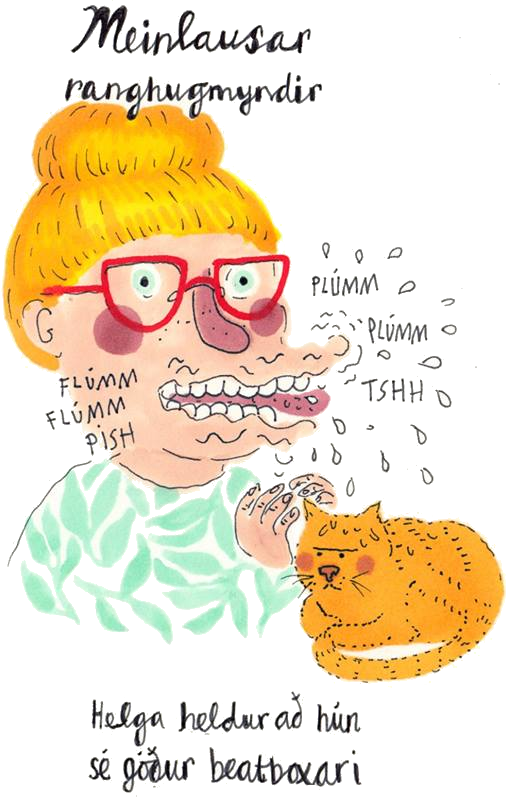
\includegraphics[width=.8\textwidth]{../figures/helga}

            \footnotesize{by Lóaboratoríum*}

            \vspace{12pt}

            \scriptsize{*not commissioned, but befitting}
        \end{column}
    \end{columns}
\end{frame}

\begin{frame}
    \frametitle{About ÍSKISUR}
    \begin{columns}[T]
        \begin{column}{0.55\textwidth}
            \begin{itemize}
                \item A literary and feline entertainment podcast*
                \item Discuss the erotic and surreal book series \emph{The Legend of the Ice People} by Margit Sandemo
                \item Each episode covers part of a book from the series and concludes with a segment on internet cats
            \end{itemize}
            \vspace{12pt}

            \centering
            
\includegraphics[width=.7\textwidth]{../figures/internet-cats}
            \tiny{via @iamlilbub}

            \scriptsize{Grumpy Cat first meeting Lil Bub\\Internet Cat Festival, 2013}
        \end{column}
        \begin{column}{0.45\textwidth}
            \centering
            
\includegraphics[width=\textwidth]{../figures/podcast_image.jpg}
            \vfill
            Birna, Kristín, and dr.~Helga\\
            \vspace{12pt}
            \footnotesize{*\emph{None of the hosts are actually cats or literary experts.}}
        \end{column}
    \end{columns}
\end{frame}

\begin{frame}
    \frametitle{Timeline for the Legend of the Ice Cat-People}
    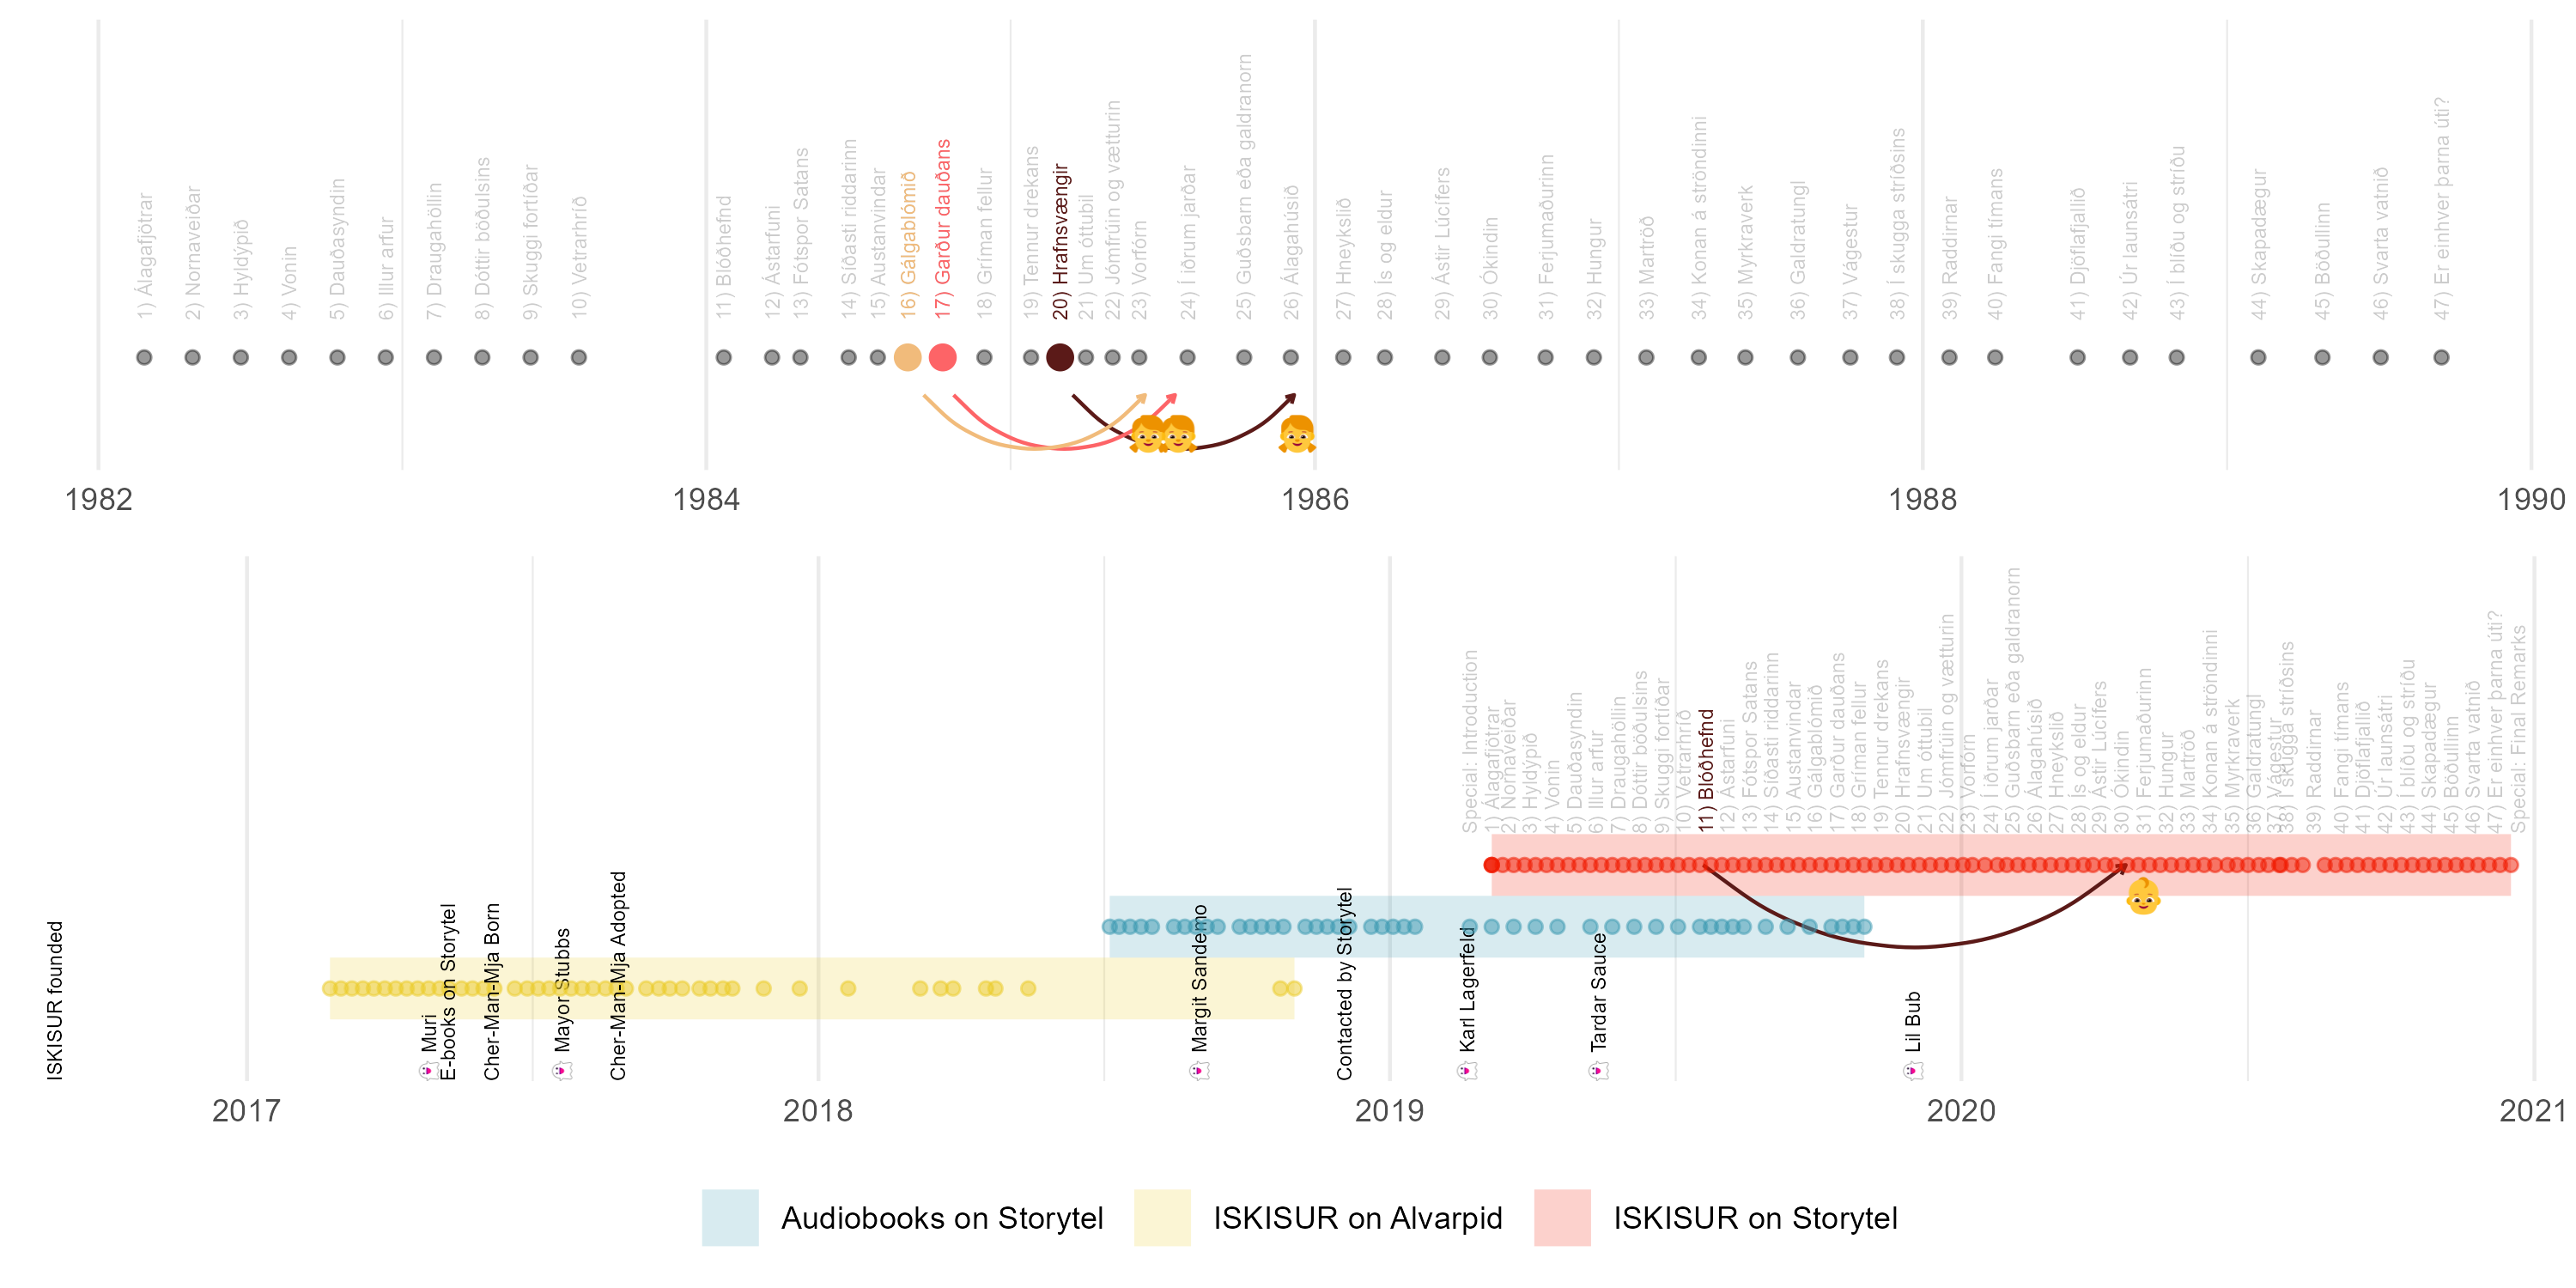
\includegraphics[width=\textwidth]{../R/figures/timeline}
\end{frame}
